\documentclass[tikz,border=0pt]{standalone}
\usepackage[T1]{fontenc}
\usepackage{lmodern}
\usetikzlibrary{shapes.symbols,calc}
\renewcommand{\familydefault}{\sfdefault}
\begin{document}
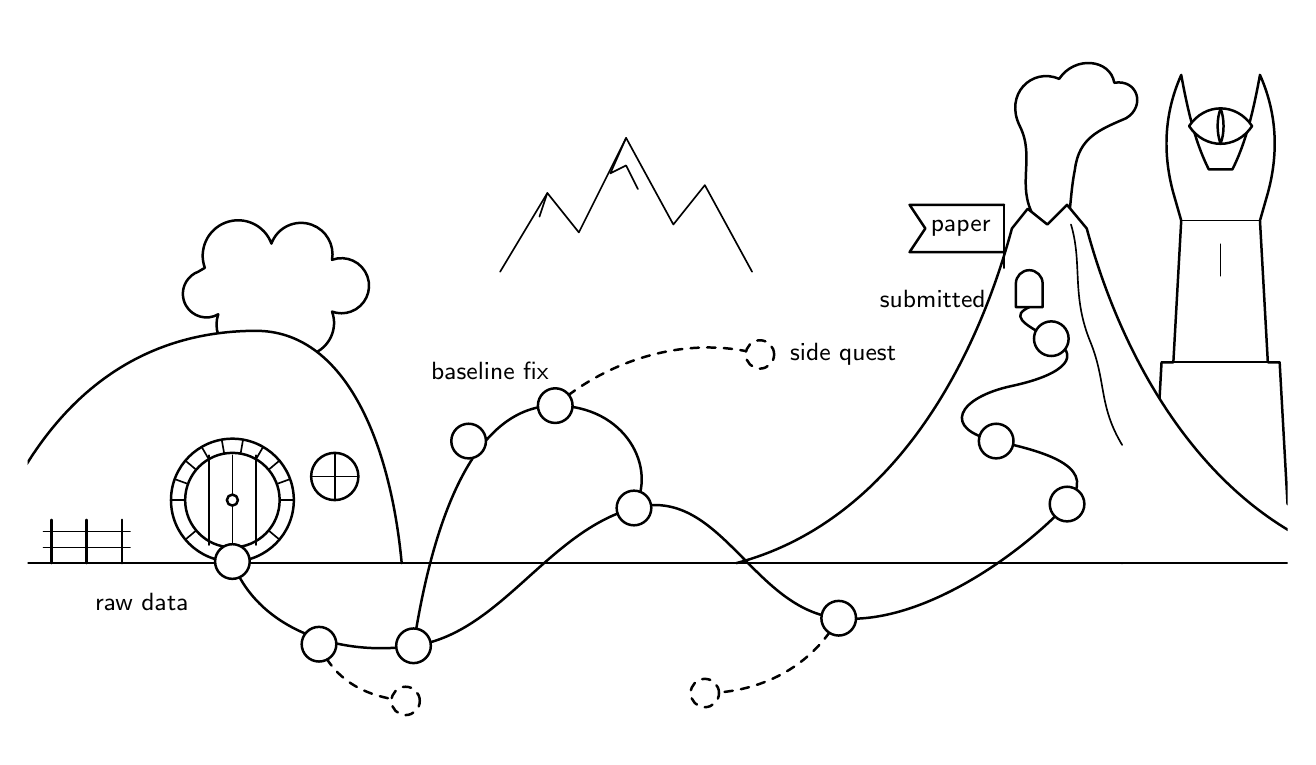
\begin{tikzpicture}[line width=0.9pt, line cap=round, line join=round, font=\sffamily,
    commit/.style={circle, draw, fill=white, minimum size=4.4mm, inner sep=0pt},
    dead/.style={circle, draw, dashed, fill=white, minimum size=3.6mm, inner sep=0pt},
    label/.style={font=\small},
    place/.style={font=\small\itshape},
    thin/.style={line width=0.6pt}]
  \clip (0,0) rectangle (16,9);

  % ================= far background: Misty Mountains =================
  \draw[thin] (6.0,5.9) -- (6.6,6.9) -- (7.0,6.4) -- (7.6,7.6) -- (8.2,6.5) -- (8.6,7.0) -- (9.2,5.9);
  \draw[thin] (7.6,7.6) -- (7.4,7.15) -- (7.6,7.25) -- (7.75,6.95);
  \draw[thin] (6.6,6.9) -- (6.5,6.6);

  % ================= Barad-dur: stepped tower, two curved horns, the Eye =================
  \draw[fill=white] (13.9,2.2) -- (14.05,2.95) -- (14.3,2.95) -- (14.4,4.75) -- (14.55,4.75)
        -- (14.65,6.55) -- (14.55,6.9) .. controls (14.4,7.45) and (14.45,7.95) .. (14.65,8.4)
        .. controls (14.75,7.85) and (14.85,7.5) .. (15,7.2)
        -- (15.3,7.2)
        .. controls (15.45,7.5) and (15.55,7.85) .. (15.65,8.4)
        .. controls (15.85,7.95) and (15.9,7.45) .. (15.75,6.9)
        -- (15.65,6.55) -- (15.75,4.75) -- (15.9,4.75) -- (16,2.95) -- (16.25,2.95) -- (16.4,2.2);
  \draw[thin] (14.65,6.55) -- (15.65,6.55);
  \draw[thin] (14.4,4.75) -- (15.9,4.75);
  \draw[thin] (15.15,5.85) -- (15.15,6.25);
  % the Eye
  \draw[fill=white] (14.75,7.75) .. controls (14.95,8.05) and (15.35,8.05) .. (15.55,7.75)
                    .. controls (15.35,7.45) and (14.95,7.45) .. cycle;
  \draw (15.15,7.53) .. controls (15.2,7.65) and (15.2,7.85) .. (15.15,7.97)
        .. controls (15.1,7.85) and (15.1,7.65) .. cycle;

  % ================= Mount Doom =================
  % smoke column drifting up and to the right
  \draw[fill=white] (12.78,6.6) .. controls (12.55,7.0) and (12.8,7.35) .. (12.6,7.75)
        .. controls (12.4,8.15) and (12.75,8.5) .. (13.1,8.35)
        .. controls (13.3,8.65) and (13.75,8.6) .. (13.8,8.3)
        .. controls (14.1,8.35) and (14.2,8.0) .. (13.95,7.85)
        .. controls (13.6,7.7) and (13.35,7.6) .. (13.3,7.2)
        .. controls (13.25,6.95) and (13.25,6.75) .. (13.22,6.6);
  % the cone: a lone, broad stratovolcano with a broken rim
  \draw[fill=white] (9.0,2.2) .. controls (10.9,2.7) and (12.0,4.6) .. (12.5,6.45)
        -- (12.7,6.7) -- (12.95,6.5) -- (13.2,6.75) -- (13.45,6.45)
        .. controls (13.95,4.6) and (15.1,2.7) .. (17.0,2.2);
  % lava runs from the crater
  \draw[thin] (13.25,6.5) .. controls (13.4,6.0) and (13.25,5.6) .. (13.5,5.0)
        .. controls (13.7,4.5) and (13.6,4.2) .. (13.9,3.7);
  % Sammath Naur: the door high on the flank
  \draw[fill=white] (12.55,5.45) -- (12.55,5.75) arc (180:0:0.17) -- (12.89,5.45) -- cycle;

  % ================= Bag End: the Hill with a round door =================
  % tree on the hill
  \draw (2.9,5.05) -- (2.9,5.75);
  \draw (2.9,5.5) -- (2.65,5.75);
  \draw[fill=white] (2.25,5.95) arc (200:20:0.45) arc (160:-10:0.4) arc (110:-110:0.35)
        arc (20:-150:0.42) arc (-30:-200:0.38) arc (-60:-250:0.3) -- cycle;
  % the hill
  \draw[fill=white] (-0.6,2.2) .. controls (0.2,4.5) and (1.6,5.15) .. (2.9,5.15)
        .. controls (4.0,5.15) and (4.6,3.8) .. (4.75,2.2);
  % round door in a stone frame, knob in the exact middle
  \draw (2.6,3.0) circle (0.78);
  \draw (2.6,3.0) circle (0.6);
  \foreach \a in {20,60,100,140,180,220,320,0,40,80,120,160}
    \draw[thin] ($(2.6,3.0)+(\a:0.6)$) -- ($(2.6,3.0)+(\a:0.78)$);
  \foreach \x in {-0.3,0,0.3} \draw[thin] (2.6+\x,2.43) -- (2.6+\x,3.57);
  \draw[fill=white] (2.6,3.0) circle (0.07);
  % round window with mullions
  \draw (3.9,3.3) circle (0.3);
  \draw[thin] (3.6,3.3) -- (4.2,3.3);
  \draw[thin] (3.9,3.0) -- (3.9,3.6);
  % garden fence
  \foreach \x in {0.3,0.75,1.2} \draw (\x,2.2) -- (\x,2.75);
  \draw[thin] (0.2,2.6) -- (1.3,2.6);
  \draw[thin] (0.2,2.4) -- (1.3,2.4);
  % ground
  \draw (-0.6,2.2) -- (16.4,2.2);

  % ================= the road: main line of commits =================
  \draw (2.6,2.22) .. controls (2.9,1.4) and (3.9,1.0) .. (4.9,1.15)
        .. controls (6.0,1.3) and (6.6,2.6) .. (7.7,2.9)
        .. controls (8.8,3.2) and (9.2,1.6) .. (10.3,1.5)
        .. controls (11.4,1.4) and (12.7,2.4) .. (13.2,2.95)
        .. controls (13.6,3.4) and (13.0,3.6) .. (12.3,3.75)
        .. controls (11.6,3.9) and (11.8,4.3) .. (12.5,4.45)
        .. controls (13.2,4.6) and (13.4,4.85) .. (13.0,5.05)
        .. controls (12.6,5.25) and (12.5,5.35) .. (12.72,5.45);

  % kept detour: branch off and merge back
  \draw (4.9,1.15) .. controls (5.2,3.1) and (5.8,4.2) .. (6.7,4.2)
        .. controls (7.6,4.2) and (8.0,3.4) .. (7.7,2.9);

  % side quests that go nowhere
  \draw[dashed] (6.7,4.2) .. controls (7.4,4.8) and (8.4,5.1) .. (9.3,4.85);
  \draw[dashed] (3.7,1.17) .. controls (3.9,0.7) and (4.3,0.5) .. (4.8,0.45);
  \draw[dashed] (10.3,1.5) .. controls (9.9,0.8) and (9.2,0.55) .. (8.6,0.55);

  % flag at the door of Sammath Naur
  \draw (12.4,5.95) -- (12.4,6.75);
  \draw (12.4,6.75) -- (11.2,6.75) -- (11.4,6.45) -- (11.2,6.15) -- (12.4,6.15);

  % ================= commits on top =================
  \node[commit] at (2.6,2.22) {};
  \node[commit] at (3.7,1.17) {};
  \node[commit] at (4.9,1.15) {};
  \node[commit] at (5.6,3.75) {};
  \node[commit] at (6.7,4.2) {};
  \node[commit] at (7.7,2.9) {};
  \node[commit] at (10.3,1.5) {};
  \node[commit] at (13.2,2.95) {};
  \node[commit] at (12.3,3.75) {};
  \node[commit] at (13.0,5.05) {};
  \node[dead] at (9.3,4.85) {};
  \node[dead] at (4.8,0.45) {};
  \node[dead] at (8.6,0.55) {};

  % ================= labels =================
  \node[label, anchor=north] at (1.45,1.95) {raw data};
  \node[label, anchor=south east] at (6.75,4.4) {baseline fix};
  \node[label, anchor=west] at (9.55,4.85) {side quest};
  \node[label] at (11.85,6.45) {paper};
  \node[label, anchor=east] at (12.3,5.55) {submitted};
\end{tikzpicture}
\end{document}
